%
% Copyright (c) 2008 Betti "Osterholz
%
% Permission is granted to copy, distribute and/or modify this document
% under the terms of the GNU Free Documentation License, Version 1.2 or
% any later version published by the Free Software Foundation;
% with no Invariant Sections, no Front-Cover Texts, and no Back-Cover Texts.
%
% A copy of the license is included in the file ``fdl.tex'' .
%

%Pfad fuer Bilder
\graphicspath{{./material_grundlagen/}}
\graphicspath{{./material_grundlagen/}{../material_grundlagen}}

\newpage
\part{Einf"uhrung in die Grundlagen}
\label{partIntroductionBasics}



\section{Grundlagen genetischer Algorithmen}

Evolution ist eines der grundlegensten Naturgesetze unseres Universums. Seit rund 3 Milliarden Jahren gibt es auf der Erde eine genetische Evolution, die, wie wohl nur wenige bestreiten werden, ganz erstaunliche Ergebnisse und Probleml"osungen hervorgebracht hat. Deshalb ist es nicht verwunderlich, dass versucht wird, die Methoden und/oder die Wirkungsweise der genetischen Evolution auch in der Informationstechnik einzusetzen. Vielfach werden schon gro"se Fortschritte in der Wissenschaft und Forschung erzielt, indem man sich Prinzipien der Ergebnisse (z. B. Fl"ugelauftrieb) der nat"urlichen Evolution von der Natur ``abgeschaut'' hat. Aber auch viele Interpretationen der Evolution wurden schon, teilweise mit Erfolg, versucht anzuwenden.

Die nachfolgende Arbeit ist einer dieser Versuche.

Wie funktioniert Evolution aber oder was ist sie "uberhaupt genau?

Ob ich diese Fragen zufriedenstellend beantworten kann, wei"s ich nicht. Ich will es aber versuchen und vielleicht noch ein paar Denkanst"o"se geben. Die nachfolgende Sicht von Evolution und genetischer Evolution ist grundlegend f"ur die gesamte vorliegende Arbeit. Sie nimmt aber keinesfalls in Anspruch, vollst"andig oder ``richtig'' zu sein. Um genetische Evolution verstehen zu k"onnen, muss wahrscheinlich zuerst erkl"art werden, was Evolution ist.


\subsection{Geschichte}

Der ber"uhmteste Forscher, der auf die Evolution aufmerksam wurde und dar"uber eine Buch verfasste, war Charles Darwin (1809- 1882), der 1859 das Buch ``Die Entstehung der Arten''\cite{EACD} ver"offentlichte. Dabei ging es um die Evolution in der Natur und wie Arten aus anderen Arten entstanden sind. Eine Idee, die ihm besonders im Kreise der damals noch wesentlich m"achtigeren Kirche viele Unsympathien einbrachte, da diese Idee dem Sch"opfungsgedanken zuwiderlief.

Die Idee, Evolution auch zum maschinellen Lernen zu verwenden, war sehr fr"uh in der Informatik vorhanden. Schon 1932 beschrieb W. D. Cannon nat"urliche Evolution als einen Lernprozess. A. M. Turing (1950) vermutete ``an obvious connection between $[$machine learning$]$ and evolution'' ("Ubersetzung: ``eine offensichtliche Verbindung zwischen $[$maschinellem Lernen$]$ und Evolution''). Leider war zu dieser Zeit die Rechnerleistung bei weitem noch nicht hoch genug, um eine Simulation der Evolution in vern"unftigem Rahmen zu gew"ahrleisten.
%TODO cite

Erst in den 1980ern war die zur Verf"ugung stehende Rechenleistung hoch genug, um Evolution zum maschinellen Lernen sinnvoll einsetzen zu k"onnen. Danach wurde das Interesse an Evolution in der Informatik gr"o"ser. Evolution wurde schon in vielen Bereichen mehr oder weniger erfolgreich eingesetzt. Angefangen vom Finden globaler/lokaler Optima von Funktionen, bis hin zum automatischem Schaltungsentwurf oder Roboterkonstruktion.


\subsection{Evolution}

Evolution ist ein allgemeines Prinzip/Naturgesetz, das man kurz mit ``Das Bessere setzt sich durch'' erkl"aren kann. Bei genauerer Betrachtung wird der Spruch etwas undeutlich, denn was ist ``besser'' (f"ur wen) und was ist ``sich'' oder ``durchsetzen''.

``Sich'' kann auf alles bezogen werden. Ob es nun ein Lebewesen, ein Programm, ein Prinzip oder Sonstiges ist. F"ur ``sich'' sind aber die Informationen die es enth"alt (z. B. Aufbau der Molek"ule oder Art des Gemeinschaftslebens) und nicht seine Materie oder Energie (wenn vorhanden) f"ur die Evolution ausschlaggebend. Ein Hund ist nicht so erfolgreich, weil er 25 Kilogramm Materie enth"alt, sondern weil diese Materie ( und seine Energie, wenn diese von Materie getrennt wird) auf ganz spezielle Weise ``verteilt/aufgebaut'' ist. Auch darf ``sich'' nicht als ein abgeschlossenes Einzelnes gesehen werden, sondern muss die Umwelt mit einbeziehen. Ameisen sind z. B. so erfolgreich, weil sie in Staaten leben. ``Sich'' kann auch weitere ``sichs'' enthalten oder in einem ``sich'' enthalten sein. So haben viele S"augetiere Darmbakterien, ohne die sie nicht mehr die gleichen Tiere w"aren. Viele Arten bestehen nur aufgrund dieser Darmbakterien, z. B. K"uhe.

Die Frage ``F"ur wen besser?'' muss mit ``F"ur sich besser'' beantwortet werden. ``F"ur sich besser'' ist, wenn ``sich'' h"aufiger oder wahrscheinlicher wird. 

Damit ist auch gleich die Frage beantwortet, was ``durchsetzen'' ist: Etwas setzt ``sich'' durch, wenn es wahrscheinlicher/h"aufiger in einer Gruppe/Menge von Dingen bzw. anderen ``sichs'' wird. Die in Australien eingef"uhrten Kaninchen haben sich in den letzten Jahrhunderten gegen"uber anderen Tierarten durchgesetzt oder innerhalb dieser Tierartengruppe (Grasfresser) sind sie auf Kosten der Anderen wahrscheinlicher/h"aufiger geworden. Damit etwas wahrscheinlicher/h"aufiger werden kann, ist nat"urlich Zeit (oder "Ahnliches) von N"oten. Das hei"st, Evolution ist ein zeitlicher Prozess.

Was bei der Erkl"arung ``Das Bessere setzt sich durch'' nicht direkt "uber die Evolution gesagt wird, ist dass das ``sich'' in mehreren "ahnlichen Kopien vorhanden sein muss, damit es ``sich'' gegen andere ``sichs'' durchsetzen kann (damit sich ein Grasfresser gegen"uber anderen durchsetzen kann, muss es davon mehrere geben). Daraus folgt unter Anderem: Um an einer Evolution teilnehmen zu k"onnen, m"ussen von ``sichs'' "ahnliche Kopien erstellt werden (z. B. durch Vermehrung) und auch mehrere dieser Kopien gleichzeitig vorhanden sein (f"ur Selektion). Nur so kann sich davon ``das Bessere'' ``durchsetzen'' und es kann immer wieder ``Besseres'' entstehen.
Zusammenfassend kann gesagt werden, dass Evolution bedeutet: ``Dinge'', die so sind, dass sie sich selbst in einer Umwelt wahrscheinlicher machen, werden wahrscheinlicher. Insofern ist Evolution trivial.

Das ``sich'' wird als \index{Individuum}Individuum bezeichnet.

Wie gut ein Individuum ist, wird als \index{Fitness}\index{Evolution!Fitness}Fitness bezeichnet.

\index{Selektion}\index{Evolution!Selektion}Selektion ist die Auswahl von Individuen, so dass die besseren Individuen wahrscheinlicher/mehr werden.

\bigskip\noindent
Technisch gesehen besteht die Evolution aus drei Komponenten oder ``S"aulen'' (siehe ``Die L"osung von Darwins Dilemma'' \cite{LDD_2007}):
\begin{enumerate}
 \item Variation: die Ver"anderung von Eigenschaften bei Individuen
 \item Selektion: Individuen mit (in ihrer jeweiligen Umwelt) besseren Eigenschaften werden bevorzugt bzw. haben eine h"ohere "Uberlebenswahrscheinlichkeit.
 \item Vererbung: Individuen geben ihre Eigenschaften an ihre Nachkommen ab.
\end{enumerate}
Alle drei Komponenten sind n"otig, denn: Ohne Variation entsteht nichts Neues, ohne Selektion kann etwas Neues nicht wahrscheinlicher werden und ohne Vererbung kann sich das Neue nicht ausbreiten.

Als eine Bedingung an die Vererbung m"usste noch gestellt werden, dass durch sie die Anzahl der Individuen erh"oht werden kann. Dadurch entstehen dann auch automatisch gr"o"sere Populationen mit einer neuen guten Eigenschaft.


\subsection{Genetische Evolution}

\bigskip\noindent
\index{Genetische Evolution}\index{Evolution!genetische}Genetische Evolution bezieht sich auf eine Evolution, in der die Gene von Lebewesen (Individuen) die Informationstr"ager darstellen (\index{Genotyp}\index{Evolution!Genotyp}Genotyp). Alle Gene eines Individuums zusammen stellen dann den Genotyp eines Individuums dar. Diese werden als ein Lebewesen ``dekodiert'' bzw. f"uhren dann zur Auspr"agung des \index{Phaenotyps}\index{Evolution!Ph"anotyps}Ph"anotyps des Individuums in der Umwelt (die Umwelt kann Auswirkungen auf den Ph"anotypen und dessen Ausbildung haben). Der Ph"anotyp wiederum bestimmt zusammen mit der Umwelt (ein Fisch an Land hat keine hohe Fitness im Verh"altnis zu Landlebewesen) die Fitness (eigentlich nur ein theoretisches Ma"s) des Individuums. Der Ph"anotyp zusammen mit der Umwelt hat Auswirkungen darauf, wie wahrscheinlich das Individuum Nachkommen zeugen wird oder wie viele Individuen ein zumindest "ahnliches Genom in Zukunft erhalten. Um so mehr Individuen "ahnliches Genom erhalten, um so wahrscheinlich wird dieses oder "ahnliche Genome in Zukunft sein.
So wird der Kreis geschlossen.

\bigskip\noindent
Am Beispiel der Evolution in der Natur:

Man nehme z. B. den Schneehasen. Dieser ist besonders gut geeignet f"ur die Evolution, weil er sich so stark vermehrt. Der Hase, das kleine, kuschelige, wei"se, hoppelnde Ding, wird Ph"anotyp genannt, also das Ph"anomen in der Natur. Die Informationen, die in seinen Genen gespeichert sind, werden Genotyp genannt. (Die Genen sind [spiralf"ormige] Molek"uhlketten im Zellkern und aber auch Gene anderswo [z. B. in den Mitochondrien].)
Genotyp und Ph"anotyp zusammen werden als Individuum bezeichnet, also der Hase als Ganzes. Mehrere Individuen, die untereinander in Beziehung stehen und sich untereinander fortpflanzen k"onnen, werden als \index{Population}Population bezeichnet. Die Gesamtheit der Genotypen einer Population wird als \index{Genpool}Genpool der Population charakterisiert. Weil die Evolution (haupts"achlich) auf die Gene bzw. den Genpool wirkt, wird sie als genetische Evolution bezeichnet.

Der Genotyp bestimmt stark den Ph"anotyp, das Aussehen des Hasen, legt den Ph"anotyp aber nicht allein fest, denn die Umwelt kann als weiterer Faktor den Ph"anotyp bestimmen. Wenn ein Hase nur wenig zu fressen bekommt, wird er nicht dick werden, ganz egal, was in seinen Genen steht: Wo nichts ist, kann auch nichts werden.
Der Genpool, also die Gesamtheit der Genotypen, ist das, was die Evolution in einer Population ver"andert oder anpasst. Wird der Ph"anotyp durch die Umwelt ge"andert, wird das meist nicht weitergegeben. Wenn ein Hase d"unn ist, weil er wenig zu fressen bekommt, k"onnen seine Kinder trotzdem dick werden. 

Es ist allerdings m"oglich, dass M"utter erworbene Immunit"aten an ihre Kinder weitergeben, z. B. mit der Muttermilch, also etwas, was eigentlich zum Ph"anotyp geh"ort und nicht zum Genotyp, da diese Immunit"at nicht in den Genen kodiert ist. Hier sieht man noch einen wichtigen Punkt der Natur: Die Ausnahme ist meist Regel.

Die Ver"anderung des Genpools geschieht allerdings "uber den Umweg der Ph"anotypen der Population. 
Unter vielen Komponenten ist die Fortpflanzung dabei die wichtigste. Um so besser der Ph"anotyp dazu geeignet ist, dass das Individuum sich fortpflanzt, um so eher wird es viele Nachkommen mit seinen Genen haben und um so wahrscheinlicher werden seine Gene in der zuk"unftigen Population anzutreffen sein.

Ein flinker Hase wird wahrscheinlicher ins geschlechtsreife Alter kommen, da er J"agern besser entkommen kann, als ein nicht so flinker Hase. Dadurch haben die flinken Hasen eine bessere Chance, sich fortzupflanzen und viele Nachkommen zu haben, als langsamere. Flinke Hasen haben auch eher Gene, die sie flinker machen als Langsamere. Dadurch werden Gene, die flink machen, eher vererbt, weshalb es ziemlich schwierig ist, Hasen mit der Hand zu fangen. (Dies wei"s ich aus eigener Erfahrung.)
Hier wird ein weiterer Punkt der Evolution sichtbar: Es geht immer um Wahrscheinlichkeiten und nicht um ``mit Sicherheit''.
Hasen die flinker als andere sind, k"onnen auch einfach das Gl"uck gehabt haben. Wenn sie beispielsweise, als sie klein waren, an einen Ort gelebt haben, wo es immer gutes Futter gab. Das gute Futter hilft ihnen sicherlich dabei, gro"s und flink zu werden. Das gute Futter ist dann also ein guter Ersatz f"ur ``flinkmachendere Gene''.
Ein Hase, der noch so gute flinkmachende Gene hat, kann trotzdem noch als kleiner Hase einem Ungl"uck oder R"auber zum Opfer fallen. Es ist nur wahrscheinlicher, dass ein Hase mit ``flinkmachenden Genen'' flink wird, l"anger lebt und mehr Nachkommen zeugt. Das ist auch ein Grund, warum Evolution nur auf viele Individuen wirkt und nicht auf ein einzelnes alleine.

Hasen, die eine bessere Chance als andere haben, sich fortzupflanzen und viele Nachkommen zu zeugen, haben eine h"ohere Fitness als andere. Das hei"st, um so fitter Hasen sind, um so wahrscheinlicher werden ihre Gene in sp"ateren Generationen anzutreffen sein.

Ein weiterer Punkt ist, dass nichts so einfach oder abgeschlossen ist, wie es zun"achst scheint. Trotz der Tatsache, dass ein Hase ein Individuum ist, kann er wiederum andere Individuen, sogar ganze Populationen, enthalten. Hasen haben Darmbakterien, die als eigenst"andige Individuen in einer Umwelt (Hasendarm) angesehen werden. Der Hase ohne seine Darmbakterien ist allerdings nicht mehr das gleiche Individuum aus evolutionstechnischer Sicht, da ohne seine Darmbakterien seine Fitness anders w"are. In diesem Fall w"are sie wahrscheinlich schlechter, weil er seine Nahrung schlechter verdauen k"onnte. Diese Darmbakterien haben ihre eigenen Gene, bzw. ihren eigenen Genotyp, und ihren eigenen Ph"anotyp. Als Population haben sie ihre eigene genetische Evolution. Auch k"onnen Gruppen von Hasen zu Individuen zusammengefasst werden, die untereinander in evolution"arer Beziehung stehen. Bei solchen ``Gruppenindividuen'' z"ahlt dann nicht mehr das "Uberleben des einzelnen Hasen aus der Gruppe, sondern nur noch das der Gruppe, bzw. dessen Genpool. So k"onnen Gene, die dazu f"uhren, dass sich einzelne Hasen nicht fortpflanzen (z. B. Gene f"ur einen Besch"utzerinstinkt, der st"arker ist als der "Uberlebensinstinkt) durchaus sinnvoll sein und erhalten bleiben, wenn sie die Fitness der Gruppe erh"ohen. 

\bigskip\noindent
Evolution wirkt auch bei vielen Vorg"angen, in denen sie gar nicht vermutet wird, z. B. hat man bei Ideen oder Programmen meist mehrere von diesen zu einem Thema und mit der Zeit setzen sich dann die ``Besseren'' (was besser ist, bestimmt die Umwelt) von diesen durch und andere, nicht so gute verschwinden.

\bigskip\noindent
Die gewollte und bewusste Anwendung in der Informatik von Wissen "uber die Evolution hei"st evolution"are Algorithmen, die der genetischen Evolution entsprechend genetische Algorithmen. Deren Grundlagen seien im Nachfolgendem beschrieben.


\subsection{Grundlagen evolution"arer Algorithmen (EA)}

Evolution"are Algorithmen arbeiten auf einer Menge (Population) von potentiellen L"osungen (Individuen), die das gegebene Problem mehr oder weniger gut l"osen bzw. der optimalen L"osung mehr oder weniger nahe kommen. Von diesen L"osungen werden dann Neue geschaffen, indem einige bis alle zuf"allig ver"andert werden. Von allen (potentiellen) L"osungen, Neue und Alte, werden dann in einem Selektionsschritt einige gel"oscht. Dabei haben weniger gute L"osungen eine h"ohere Wahrscheinlichkeit gel"oscht zu werden. Dies f"uhrt im Allgemeinen dazu, dass die guten L"osungen eine h"ohere ``"Uberlebenschance'' (Fitness), also eine h"ohere Wahrscheinlichkeit, nicht gel"oscht zu werden, haben und damit in der Menge bessere L"osungen zunehmen. Diesen Prozess der Ver"anderung und Selektion wird dann solange wiederholt, bis eine Endbedingung (Terminalkondition) zutrifft. Die Endbedingung ist meist: Eine bestimmte Anzahl von Durchl"aufen wurde ausgef"uhrt oder/und eine L"osung "uberschreitet eine festgelegte Grenze (z. B. wenn die L"osung gut genug ist).

\begin{lstlisting}[ numbers=left, frame=single, caption={Allgemeiner Algorithmus}, label={AllgAlgo},breaklines,basicstyle=\footnotesize\ttfamily,numberstyle=\tiny,extendedchars=true]
Initialisieren der Menge der potentiellen Loesungen
loop
  - hinzufuegen neuer Individuen zur Menge, die aus alten 
     Individuen, aus der Menge, mit Zufall generiert werden
  - Selektion = zufaelliges Loeschen von Individuen aus der 
     Menge, bessere haben eine hoehere Wahrscheinlichkeit,
     nicht geloescht zu werden
until (Terminalkondition erfuellt)
\end{lstlisting}

Im Listing \ref{AllgAlgo} ist schematisch der allgemeine Algorithmus eines evolution"aren Algorithmus in pseudo-C dargestellt.

%TODO
%Der gleiche Algorithmus wird im Bild \ref{bAllgAlgo} grafisch dargestellt.
%\begin{figure}[htbp]
%\begin{center}
%  \includegraphics[scale=0.7]{Iteratio.jpg}
%\end{center}
%\caption{Allgemeiner Algorithmus}
%\label{bAllgAlgo}
%\end{figure}

%\begin{figure}[htbp]
%\begin{center}
%  \includegraphics[scale=0.7]{WeelSel.jpg}
%\end{center}
%\caption{weel-selection}
%\label{WeelSel}
%\end{figure}

Bei der Selektion von Individuen findet oft die weel-selection Anwendung.
%TODO: , dargestellt in Bild \ref{WeelSel} ("ubernommen aus \cite{GEA}). 
Dabei haben L"osungen/Individuen mit einer niedrigeren Fitness eine h"ohere Wahrscheinlichkeit, gel"oscht zu werden. Der Name weel-selection hat seinen Ursprung darin, dass Wahrscheinlichkeiten f"ur Individuen grafisch in einem Kreis angeordnet werden k"onnen (Individuen mit geringerer Fitness bekommen einen gr"o"seren Kreisausschnitt). Auf diesem Kreis (bzw. seinem Rand) wird bei der Selektion zuf"allig ein Punkt ausgew"ahlt und das zugeh"orige Individuum gel"oscht.


\subsection{Unterarten}

Es werden zwei Arten von evolution"aren Algorithmen unterschieden. Die Evolutionsstrategien und die genetische Algorithmen (GA), wobei diese noch in weitere Unterarten unterschieden werden kann (z. B. sequentielle und parallele oder klassische GA und genetische Programmierung).
Eine m"ogliche Einteilung ist in der Abbildung \ref{genAbst}  (nach \cite{GEA}), dabei sind die evolution"aren Algorithmen neben den Simulated Annealing als eine Unterart der informellen Zufallssuche eingeordnet.

Wo denn nun genau diese Unterschiede der Arten liegen, ist oft nicht mehr so klar zu erfassen:
\cite{ECDF00} ``Within the past five years, each area of evolutionary computation has borrowed and modified ideas from the others. Over time, an iterative blending has occurred such that all classes of evolutionary algorithms now appear quite similar, if not for all intents and purposes identical''
Eine genaue Einteilung von realisierten Algorithmen in die verschiedenen Arten ist also nicht so leicht m"oglich.


\begin{figure}[htbp]
\begin{center}
  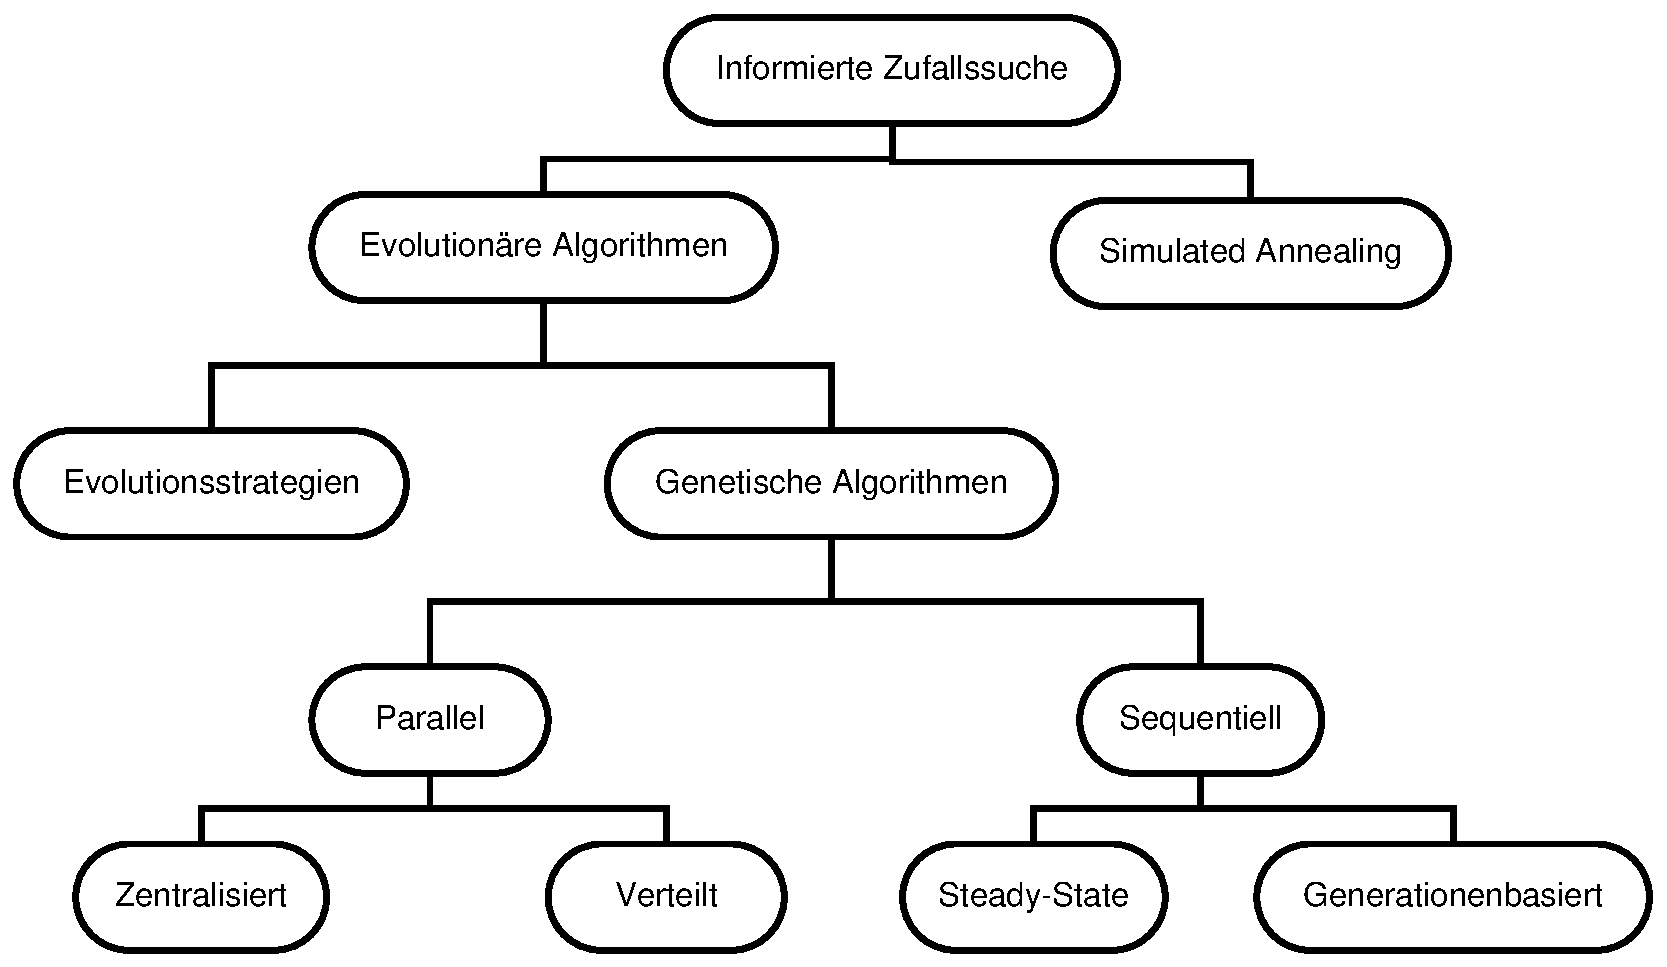
\includegraphics[scale=0.4]{unterteilung_EA_GA.eps}
\end{center}
\caption{Einteilung von Lernverfahren}
\label{genAbst}
\end{figure}


\subsubsection{Genetische Algorithmen (GA)}

Genetische Algorithmen k"onnen einfach beschrieben werden als: evolution"are Algorithmen + ``Crossover''

Vorbild: nat"urliche Evolution auf Genbasis

Dabei wird als ``Crossover'' der Vorgang bezeichnet, bei dem von zwei oder mehr Individuen die (Erb-)Informationen kombiniert werden, um ein neues Individuum zu schaffen.

\subsubsection{Klassische genetische Algorithmen (GA)}

Die klassischen genetische Algorithmen (GA) sind Algorithmen die auf einer Liste mit Bits arbeiten, welche die potentiellen Probleml"osungen/Individuen repr"asentieren. Mutation ist dabei das Invertieren von Bits. Beim Crossover gibt es meist one- oder two-point-crossover (bei GA's). Beim one-point-crossover wird die Bitsequenz der beiden Individuen jeweils an einem Punkt, meist die gleiche Position, durchgeschnitten und die beiden Teilh"alften eines Individuums mit den entsprechend anderen Teilh"alften des anderen Individuums verbunden. Two-point-Crossover ist identisch, nur das hier an zwei Punkten geschnitten wird.

%TODO
%Die Arbeitsweise von one-point-crossover ist in Bild \ref{onePCO} gezeigt, die von two-point-crossover im Bild \ref{twoPCO}  (beide "ubernommen aus \cite{GEA}).
%\begin{figure}[htbp]
%\begin{center}
%  \includegraphics[scale=0.5]{onePCO.jpg}
%\end{center}
%\caption{one-point-crossover}
%\label{onePCO}
%\end{figure}

%\begin{figure}[htbp]
%\begin{center}
%  \includegraphics[scale=0.5]{twoPCO.jpg}
%\end{center}
%\caption{two-point-crossover}
%\label{twoPCO}
%\end{figure}


\subsection{Anmerkungen zu evolution"aren Algorithmen (EA)}

Eine geeignete Wahl der Repr"asentation von L"osungen (also wie die Individuen aufgebaut sind) und angepasste Operatoren (welche die Individuen ver"andern bzw. neue Individuen erzeugen) k"onnen die Performance von evolution"are Algorithmen deutlich erh"ohen (\cite{ECDF00}).
Durch eine geeignete Wahl der Repr"asentation wird der Hypothesenraum, den diese aufspannen, g"unstig beeinflusst, z. B. k"onnen ung"ultige oder unerw"unschte L"osungen ganz entfallen. Weiterhin erm"oglicht eine gute Repr"asentation auch einen Hypothesenraum, in dem Operatoren einfacher zu realisieren sind, die im Allgemeinen schneller zur L"osung f"uhren, z. B. ist es dann wahrscheinlicher, dass "ahnliche L"osungen auch nahe im Hypothesenraum ``beieinanderliegen'' (f"ur die Operatoren).

Durch angepasste Operatoren werden die ``Wege'' (welche diese Operatoren im Hypothesenraum erzeugen) besser, bzw. f"uhren schneller zu besseren L"osungen. Es k"onnen beispielsweise als Operatoren schon bekannte Algorithmen zur Optimierung eingesetzt werden oder es kann in den Operatoren Wissen "uber das Problem verwendet werden.

Die gro"se Freiheit bei der Wahl der Repr"asentation der potentiellen Probleml"osung ist einer der gr"o"sten Vorteile der evolution"aren Algorithmen. Theoretisch ist eine beliebige Repr"asentation w"ahlbar, solange eine Bewertung von potentiellen Probleml"osungen in dieser m"oglich ist. Andere Lernverfahren erm"oglichen meist nur bestimmte Repr"asentationen, z. B. k"onnen Lernverfahren von neuronalen Netzen nur neuronale Netze als Probleml"osung hervorbringen. Bei EAs allerdings k"onnen unter anderen Bitlisten, Molek"ule, beliebige Programmiersprachen oder mathematische Formeln verwendet werden. Genauso variabel sind damit auch die Operatoren, mit denen die potentiellen L"osungen angepasst werden k"onnen. Damit k"onnen viel besser Vorwissen oder auch Vermutungen in den Algorithmus eingearbeitet werden.

Weiterhin kann bei der Wahl der Repr"asentation auch noch die Anschaulichkeit f"ur den Menschen ber"ucksichtigt werden. Das hei"st, die Repr"asentation kann so gew"ahlt werden, dass potentielle Probleml"osungen einfacher verstanden werden k"onnen.

Der gro"se Nachteil von evolution"aren Algorithmen ist der hohe Zeitaufwand bzw. Rechenaufwand den sie im Verh"altnis zu anderen Algorithmen ben"otigen. Wo andere Algorithmen die vorhanden Daten nutzen, um aus ihnen einmal eine L"osung zu generieren, generiert ein genetischer Algorithmus st"andig neue L"osungen, testet, wie gut diese sind, und w"ahlt m"oglichst die Guten aus. Solange die Terminalkondition nicht erf"ullt ist, h"alt ein genetischer Algorithmus auch nicht an. Die Terminalkondition kann aber auch sehr schwer oder gar nicht erf"ullbar sein. Ein gutes Beispiel ist auch hier die nat"urliche Evolution: Sie l"auft schon seit mindestens 4 Milliarden Jahren auf wenigstens einen ganzen Planeten, und es ist noch kein Ende abzusehen.


\section{Multimediaformate}

Multimedia ist der Begriff f"ur Informationen, wenn mehrere Medien geb"undelt werden. Medien sind Tr"ager von Dingen, die "uber Sinne wahrnehmbar sind, wobei den verschiedenen Sinnen jeweils ein Medium zugeordnet ist.
Multimediaformate sind danach S"atze von Regeln, wie diese Dinge abgespeichert (dauerhaft gemacht) oder "ubertragen werden k"onnen.

\bigskip\noindent
Dabei sind unter Anderem Medien f"ur folgende Dinge zu unterscheiden:
\begin{itemize}
\item Bild
\item Ton
\item olefaktorische Medien (Ger"uche)
\item hauptische Medien (wie sich ein Gegenstand anf"uhlt, z. B. hart oder rau)
\end{itemize}

Im Nachfolgenden werden vor Allem das Bild und der Ton beschrieben, da sie die gr"o"sten Bereiche sind (bzw. in unser heutigen Informationsgesellschaft am h"aufigsten anzutreffen sind).

\subsection{Bilder}

\subsubsection{Einleitung}

Wie auch in vielen anderen Bereichen wurde mit dem Aufkommen leistungsf"ahiger Computer die Bildverarbeitung revolutioniert. Handelte es sich Anfang der 60er Jahre \cite{projBildf}, als die grafische Datenverarbeitung aufkam, noch haupts"achlich um Strichzeichnungen und Diagramme, die erstellt, manipuliert und verarbeitet wurden, so sind es heutzutage ganze Filme, die mit Computern erzeugt werden. Es ist schon heute so gut wie unm"oglich, ein durch gute Manipulationen erstelltes Bild von einem ``echten'' (nicht manipuliertem) Bild zu unterscheiden.
Heute stehen eine Unzahl von Programmen zur Erstellung, Manipulation und Verarbeitung von Bildern zur Verf"ugung und damit einhergehend eine Unzahl von Bildformaten. Alle diese Bildformate haben ihre Vor- und Nachteile und werden in den verschiedensten Bereichen genutzt.

Im Nachfolgenden sollen einige wichtige Eigenschaften von Bildkodierungen n"aher erl"autert werden.

\subsubsection{Bildformat}

Ein Bildformat oder Bildkodierung ist ein Format (bzw. eine Strukturbeschreibung) f"ur eine Ansammlung von Daten, die ein Bild repr"asentieren. Dabei kommt es vor Allem auf die effiziente Organisation der Daten in Bezug auf das Anwendungsgebiet an. Die meisten Bildformate teilen ihre Daten in zwei Bl"ocke auf: einen Block mit allgemeinen Informationen zum Bild (Farbpalette, Bildgr"o"se, etc.) und einen Block der angibt, was auf dem Bild dargestellt wird (z. B. die Objekte oder die Farbwerte f"ur die einzelnen Pixel).
In Bild \ref{DatBit} ist als Beispiel der Aufbau einer Datei im Bitmapformat BMP (*.bmp) angegeben. Eingeleitet wird dieses Format durch den Bitmap Header, der anzeigt, dass es sich um ein Bitmapbild handelt (er besteht aus den Buchstaben ``bmp''). Im Informations-Header befinden sich Informationen zum Bild selbst, unter anderem sind dort zu finden: die H"ohe und Breite des Bildes, die horizontale und vertikale Aufl"osung in Pixel pro Meter, der Typ der Komprimierung und die Anzahl der benutzten Farben.

Die Farbpalette definiert jede Farbe durch ihren Anteil an Rot, Gr"un und Blau.
Die Daten enthalten die zeilenweise Rasterinformation des Bildes. Hierbei ist der
Ausgangspunkt die linke untere Ecke des Bildes.

\begin{figure}[htbp]
\begin{center}
\begin{picture}(5,4.5)
	\linethickness{4pt}
	\put(0,3){\framebox(4,1){Bitmap Header}}
	\put(0,2){\framebox(4,1){Informations-Header}}
	\put(0,1){\framebox(4,1){Farbpalette}}
	\put(0,0){\framebox(4,1){Daten}}
\end{picture}
\end{center}
\caption{Dateiaufbau eines Bitmap-Bildes}
\label{DatBit}
\end{figure}


\subsubsection{Eigenschaften von Bildern}

Wichtige Eigenschaften f"ur Bildformate werden im Folgendem aufgef"uhrt. Dabei m"ussen nicht alle Bildformate alle Eigenschaften unterst"utzen.

Der \textbf{Dateityp} (Filetype) ist das, woran im Dateisystem erkannt werden kann (oder zumindest erkannt werden sollte), um welche Art von Bildkodierung es sich handelt. Meist handelt es sich dabei um ein Dateiendungsk"urzel, das eine Art Abk"urzung der vollen Bezeichnung der Bildkodierungsart ist, z. B. die Dateiendung ``.bmp'' f"ur die Bitmap-Kodierung.

\bigskip\noindent
Die \textbf{maximale Bildgr"o"se} gibt an, wie die maximale Gr"o"se eines Bildes sein darf, um in diesem Bildformat noch abspeicherbar zu sein. Typisch ist hier die maximale Anzahl der Pixel, die ein Bild haben darf.
Die maximale Bildgr"o"se h"angt vom Speicherformat ab. Da in digitalen Rechnern nicht unendlich gro"se Zahlen abgespeichert werden k"onnen (wegen des begrenzten Speicherplatzes), k"onnen auch die Zahlen f"ur Koordinaten oder Bildgr"o"se nur endlich sein.

\bigskip\noindent
Die \textbf{Anzahl der Kan"ale} gibt an, aus wie vielen Teilbildern "ubereinander das Bild besteht. "Ublich ist ein Kanal, aber in einigen Anwendungen ist es notwendig, mehrere Bilder "ubereinander zu legen, um z. B. besser Transparenzen im Bild darstellen zu k"onnen.

\bigskip\noindent
Mit dem \textbf{Farbmodell} werden die Farben angegeben, die verwendet werden k"onnen. Der einfachste Fall ist z. B. S/W (nur schwarz und wei"s als ``Farben'').

\bigskip\noindent
Die \textbf{Farbtiefe} geh"ort zum Farbmodell und ist die Anzahl m"oglichen Farben, die einem Pixel oder Objekt zugeordnet werden k"onnen.
Farbtiefe in Bits ist die Anzahl der Bits pro Farbe, die einem Pixel oder Objekt f"ur dessen Farbe zugeordnet werden.
Die beiden Begriffe h"angen eng zusammen, da die Bits pro Farbe meist die Farbtiefe bestimmen nach der Formel: $Farbtiefe = 2 ^ {(Bits\ pro\ Farbe)}$

\bigskip\noindent
Der \textbf{Hersteller} eines Bildformates ist wichtig im Hinblick auf Lizenzen und m"ogliche Updates. Muss f"ur ein Bildformat bezahlt werden, wenn es in einer Software benutzt werden soll? Wird dieses Bildformat in Zukunft eventuell noch besser ausgebaut usw. ?

\bigskip\noindent
\textbf{Plattformabh"angigkeit}: Bei vielen unbekannteren Bildformaten gibt es nur f"ur einige Plattformen (z. B. Rechnertypen oder Betriebsysteme) Programme zum Erstellen, Bearbeiten oder Darstellen von Bildern in ihnen.

\bigskip\noindent
Als \textbf{Komprimierung} wird bezeichnet, wie viel Informationen (Bits) f"ur ein Bild ben"otigt werden, um es aus diesen wiederherzustellen.

\bigskip\noindent
Die \textbf{Darstellungsarten} Vektorgrafik oder Rastergrafik beziehen sich auf die Art, wie die Bildinformationen abgespeichert sind. Bei Rastergrafiken wird "uber das Bild ein Raster gelegt und die einzelnen Punkte abgespeichert. Bei Vektorgrafik werden die ``Objekte'' (z. B. Linien, Kreise) des Bildes abgespeichert.


\subsubsection{Kodierungen in den Darstellungsarten Vektorgrafik oder Rastergrafik}

\paragraph{Vektorgrafik:}

Bei der Vektorgrafik werden die Daten f"ur einzelne Objekte (dessen ``Vektoren'') gespeichert. Der Vektorgrafiktyp bestimmt die m"oglichen Objekte. Oft finden daf"ur Punkte, Linien und Kreise Verwendung. Der Vektorgrafiktyp, und damit die verwendeten Objekte, orientieren sich meist stark an dem Anwendungsgebiet, f"ur das dieser Vektorgrafiktyp geschaffen wurde, z. B. technischer Entwurf von Geb"auden oder Ger"aten. Die Objekte werden mathematisch durch eine Anzahl von Werten definiert, z. B. Anfangsposition, L"ange oder Radius. Vektorgrafiken sind vor allem bei technischen Zeichnungen verbreitet (z. B. CAD-Systeme).

\bigskip\noindent
Vorteile:
\begin{itemize}
  \item Grafikobjekte k"onnen (meist) ohne Qualit"atsverlust verschoben, skaliert oder mit Farbe versehen werden.
  \item Ein Vektorbild besteht aus vielen verschiedenen Einzelobjekten, die sich bei Ver"anderungen gegenseitig nicht beeinflussen.
  \item Im Vergleich zu Rastergrafiken wird hier meist weniger Speicherplatz ben"otigt, da eine geringere Anzahl von Informationen gespeichert wird (z. B. einen Kreis als Matrix/Raster aus Farbwerten zu beschreiben, wie bei der Rastergrafik, ist aufwendiger, als einen Kreis mit Mittelpunkt und Radius zu beschreiben).
  \item Die Vektorgrafiken sind (meist) nicht an eine bestimmte Aufl"osung gebunden, d. h. sie passen sich den M"oglichkeiten des Ausgabeger"ats an.
\end{itemize}


\bigskip\noindent
Nachteile:
\begin{itemize}
  \item	Zur Bildschirm- und Druckerausgabe m"ussen die Vektorgrafiken gerastert werden, da diese Ger"ate nur Punkte darstellen k"onnen. Ein Treppeneffekt ist die Folge.
  \item	Eine direkte Umwandlung von Rastergrafik oder Vektorgrafiken eines Typs in eine Vektorgrafik anderen Typs ist meist nur schwer und mit viel Aufwand zu realisieren. (Bei Vektorgrafiken geht es darum, die Objekte des Bildes darzustellen. Wie findet man aber solche bei Rastergrafiken? Einfach jeden Punkt als Objekt [z. B. als Rechteck] zu deklarieren, w"urde keinen der oben genannten Vorteile bringen.)
  \item	Die meisten Bilder liegen nach dem Einlesen in einem Rastergrafikformat vor.
\end{itemize}


\paragraph{Rastergrafik:}

Bei der Rastergrafik (auch Bitmapgrafik) wird "uber das Bild ein Raster gelegt und die einzelnen Punkte bzw. ihre Farbe (im Farbmodell) abgespeichert. Damit besteht ein Rasterbild aus einer Menge von Pixeln (Bildpunkten), die eine bestimmte Farbe haben. Bei gen"ugend vielen Pixeln pro Fl"ache und gen"ugend Farben kann das menschliche Auge die einzelnen Pixel nicht mehr wahrnehmen und es entsteht der Effekt eines ``fotorealistischen'' Bildes.

\bigskip\noindent
Vorteile:
\begin{itemize}
  \item	einfaches Abspeichern von Bildern, es m"ussen keine Objekte bekannt sein
  \item	Da die meisten Ger"ate (z. B. Monitor, Scanner, Drucker) zum Darstellen oder Einlesen von Bildern mit Rastern arbeiten, ist die Umwandlung in oder von Rastergrafiken f"ur diese Ger"ate einfach.
\end{itemize}

\bigskip\noindent
Nachteile:
\begin{itemize}
  \item	Da jeder einzelne Punkt eines Bildes abgespeichert wird, kostet es meist viel Speicherplatz.
  \item	Bei einer starker Vergr"o"serung eines Rastergrafikbildes kommen die einzelnen Pixel zum Vorschein und die Grafik wirkt eckig.
  \item	Objekte des Bildes k"onnen nur noch schwer oder gar nicht automatisch identifiziert werden.
\end{itemize}

\subsubsection{Farbmodell/Farbschema}

Das Farbmodell gibt an, wie die Farben im Bild dargestellt werden. Es handelt sich bei diesen Farben um einen Vektor mit diskreten (z. B. ganzen) Zahlen aus einem Definitionsbereich. Dieser Vektor wird dann jeweils einem Pixel oder einem anderem Objekt (bei Vektorgrafik) zugeordnet. Der Darstellbarkeit wegen werden Schwarz und Wei"s auch als Farben angesehen. Ihnen ist im allgemeinen auch ein Vektor zugeordnet.
Die Anzahl der Farben, die ein Bild haben kann, wirkt sich stark auf die Gr"o"se des n"otigen Speichers f"ur dieses aus.

\bigskip\noindent
Im Nachfolgenden sind einige bekannte Beispiele aufgef"uhrt.

\paragraph{S/W (schwarz/wei"s):}

Das S/W-Farbmodell (S/W steht dabei f"ur schwarz/wei"s) ist wohl das "alteste, einfachste und am wenigsten speicheraufw"andige Farbmodell. Dabei wird pro Objekt (z. B. pro Pixel) ein Bit gespeichert, das je nach Wert (z. B. wei"s = true, schwarz = false) angibt, ob das Objekt (z. B. der Punkt) wei"s oder schwarz sein soll bzw. heller oder dunkler darzustellen ist, z. B. f"ur Monitore die kein wirkliches Schwarz oder Wei"s darstellen k"onnen.


\paragraph{Grayscale (Halbton):}

Beim Grayscale werden 256 Abstufungen von schwarz bis wei"s unterschieden. Pro Objekt werden daf"ur ein Byte oder acht Bit abgespeichert. Dies wird dann als eine dieser Abstufungen interpretiert.


\paragraph{RGB:}

Das RGB-Farbmodell ist ein additives Verfahren, mit den drei Grundfarben Rot, Gr"un und Blau. Jeder dieser Grundfarben ist ein Wert zugeordnet: Umso gr"o"ser dieser ist, desto heller ist der entsprechende Anteil dieser Grundfarbe in der erzeugten Farbe. %, dargestellt in Bild \ref{RGB} ("ubernommen aus \cite{projBildf}). 
Mit diesem Farbmodell k"onnen alle Farben mit einer Genauigkeit dargestellt werden, die mit der Definitionsbereichsgr"o"se der einzelnen Farben ansteigt.
Das Farbmodell hat seinen Ursprung in der Realisierung von Farben auf Monitoren (Braunsche R"ohren), da auch dort nur drei verschiedenfarbige Punkte zu einem Pixel zusammenfasst werden: Je st"arker der Elektronenstrahl einen dieser Punkte anstrahlt, desto heller erscheint er in seiner Farbe. Daher eignet sich dieses Farbmodell auch besonders gut f"ur diese Monitordarstellungen, es muss nicht mehr viel umgerechnet werden.

%TODO
%\begin{figure}[htbp]
%\begin{center}
%  \includegraphics[scale=0.5]{RGBFarb.jpg}
%\end{center}
%\caption{additives Farbschema}
%\label{RGB}
%\end{figure}
 
\paragraph{Indizierte Farben:}

Bei indizierten Farben wird nicht immer der gleiche ``Farb\-raum'' f"ur jedes Bild verwandt, sondern je nach Bild, je nach dem welche Farben bei ihm ben"otigt werden, nur diese Farben oder "ahnliche. Jede dieser Farben bekommt eine ``Nummer'' (Indices), die in einer Tabelle der wirklichen Farbe (z. B. im RGB-Farbmodell) zugeordnet wird. Da im Bild nun viel weniger Farben dargestellt werden m"ussen, wird Speicherplatz gespart. 

\subsubsection{Komprimierung}

Bei der Komprimierung geht es darum, Speicherplatz f"ur ein Bild zu sparen. Umso weniger Speicherplatz ein Speicherformat f"ur ein Bild ben"otigt, desto h"oher wird der Kompressionsfaktor dieses Speicherformats angesehen. Ein h"oherer Kompressionsfaktor eines Speicherformats f"uhrt meist zu einen h"oheren Kompressionsfaktor eines in ihm abgespeicherten Bildes. Leider ist die Festlegung, f"ur welches Speicherformat der Kompressionsfaktor null ist, mehr oder weniger willk"urlich, denn es k"onnen immer zu einem Speicherformat weitere Informationen "uber das abgespeicherte Bild hinzugef"ugt (z. B. Redundanzen, History) und der Kompressionsfaktor verschlechtert werden.
Der Ausdruck ein Bild sei ``unkomprimiert'' ist somit nicht zutreffend. Zutreffender ist, dass solche Bilder einen niedrigen Kompressionsgrad haben.

\bigskip\noindent
Es werden zwei gro"se Komprimierungsarten unterschieden.

\paragraph{Verlustfreie Komprimierung:}

Dabei gehen keine Informationen "uber das Bild verloren. Das hei"st, wenn ein Bild mit einem verlustfreien Verfahren komprimiert und danach wieder hergestellt wird, ist das Abbild mit dem Original identisch.

\paragraph{Verlustbehaftete Komprimierung:}

Dabei gehen Informationen "uber das Bild verloren. Das hei"st, wenn ein Bild mit einem verlustbehafteten Verfahren komprimiert und danach wieder hergestellt wird, ist das Abbild mit dem Original nicht mehr identisch. Es k"onnen z. B. Pixel mit einer leicht abweichenden Farbe im Abbild vorhanden sein.

In dieser Komprimierungsart sind meist h"ohere Komprimierungsfaktoren m"oglich als mit der verlustfreie Komprimierung.


\subsection{Ton}

T"one sind Schwingungen. Die Schwingung kann dabei durch unterschiedliche Medien (z. B. Luft oder Wasser) "ubertragen werden. T"one setzen sich aus elementaren Schwingungen mit unterschiedlichen Frequenzen, Amplituden, Anfangszeitpunkten und Dauer zusammen.

Deutlich wird dies beispielsweise beim Klavierspielen. Wenn ein Klavierst"uck gespielt wird, werden die Tasten des Klaviers zu einer bestimmten Zeit gedr"uckt, woraufhin ein Ton einer bestimmten L"ange erklingt. Dieser Ton ist aus unterschiedlichen Frequenzen zusammengesetzt und hat eine bestimmte Lautst"arke, welche durch die Amplituden der Frequenzen bestimmt wird.

\bigskip\noindent
T"one k"onnen demnach abgespeichert werden indem die Schwingungen des Tons aufgezeichnet werden oder die Frequenzen.

Werden die Schwingungen des Tons aufgezeichnet (wie z. B. beim wav-Format), h"angt die Quallit"at von der Dichte der Aufzeichnungspunkte ab. F"ur jeden Aufzeichnungspunkt wird die Amplitude gespeichert. Werte von 44000 Aufzeichnungspunkten pro Sekunden sorgen f"ur einen Ton in einer guten Qualit"at. Da pro Aufzeichnungspunkt ein paar Bytes (f"ur die Amplitude) verbraucht werden, ist der Speicherbedarf relativ hoch (allein bei $2$ Bytes f"ur die Amplitude $44000 \frac{1}{s} * 2 Byte = 88000 Byte/s$, bei einer Aufzeichnung von nur 3 Minuten sind das rund 15,1 MB). Dieser Speicherbedarf verdoppelt sich noch, wenn die Aufzeichnung in Stereo gemacht werden soll.

Mit dem Abspeichern der Frequenzen von T"onen k"onnen im Allgemeinen bessere Komprimierungsraten erreicht werden. Diese kann noch gesteigert werden, wenn Frequenzen, die der Mensch normalerweise nicht wahrnimmt, nicht mit abgespeichert werden (wie z. B. beim MPEG-Audio [z. B. mp3]). Diese Art des Abspeicherns ist aber auch rechenaufw"andiger.


%TODO
%\section{Weitere Medien}
%\subsection{Olifaktorische Medien}
%\subsection{Hauptische Medien}




